\documentclass[runningheads]{llncs}

% ---------------------------------------------------------------
% Include basic ECCV package
 
% TODO REVIEW: Insert your submission number below by replacing '*****'
% TODO FINAL: Comment out the following line for the camera-ready version
\usepackage[review,year=2024,ID=*****]{eccv}
% TODO FINAL: Un-comment the following line for the camera-ready version
%\usepackage{eccv}

% OPTIONAL: Un-comment the following line for a version which is easier to read
% on small portrait-orientation screens (e.g., mobile phones, or beside other windows)
%\usepackage[mobile]{eccv}


% ---------------------------------------------------------------
% Other packages

% Commonly used abbreviations (\eg, \ie, \etc, \cf, \etal, etc.)
\usepackage{eccvabbrv}

% Include other packages here, before hyperref.
\usepackage{graphicx}
\usepackage{booktabs}

% The "axessiblity" package can be found at: https://ctan.org/pkg/axessibility?lang=en
\usepackage[accsupp]{axessibility}  % Improves PDF readability for those with disabilities.


% ---------------------------------------------------------------
% Hyperref package

% It is strongly recommended to use hyperref, especially for the review version.
% Please disable hyperref *only* if you encounter grave issues.
% hyperref with option pagebackref eases the reviewers' job, but should be disabled for the final version.
%
% If you comment hyperref and then uncomment it, you should delete
% main.aux before re-running LaTeX.
% (Or just hit 'q' on the first LaTeX run, let it finish, and you
%  should be clear).

% TODO FINAL: Comment out the following line for the camera-ready version
\usepackage[pagebackref,breaklinks,colorlinks]{hyperref}
% TODO FINAL: Un-comment the following line for the camera-ready version
%\usepackage{hyperref}

% Support for ORCID icon
\usepackage{orcidlink}


\begin{document}

% ---------------------------------------------------------------
% TODO REVIEW: Replace with your title
\title{Author Guidelines for ECCV Submission} 

% TODO REVIEW: If the paper title is too long for the running head, you can set
% an abbreviated paper title here. If not, comment out.
\titlerunning{Abbreviated paper title}

% TODO FINAL: Replace with your author list. 
% Include the authors' OCRID for the camera-ready version, if at all possible.
\author{First Author\inst{1}\orcidlink{0000-1111-2222-3333} \and
Second Author\inst{2,3}\orcidlink{1111-2222-3333-4444} \and
Third Author\inst{3}\orcidlink{2222--3333-4444-5555}}

% TODO FINAL: Replace with an abbreviated list of authors.
\authorrunning{F.~Author et al.}
% First names are abbreviated in the running head.
% If there are more than two authors, 'et al.' is used.

% TODO FINAL: Replace with your institution list.
\institute{Princeton University, Princeton NJ 08544, USA \and
Springer Heidelberg, Tiergartenstr.~17, 69121 Heidelberg, Germany
\email{lncs@springer.com}\\
\url{http://www.springer.com/gp/computer-science/lncs} \and
ABC Institute, Rupert-Karls-University Heidelberg, Heidelberg, Germany\\
\email{\{abc,lncs\}@uni-heidelberg.de}}

\maketitle


\begin{abstract}
  The abstract should summarize the contents of the paper. 
  LNCS guidelines indicate it should be at least 70 and at most 150 words.
  Please include keywords as in the example below. 
  This is required for papers in LNCS proceedings.
  \keywords{First keyword \and Second keyword \and Third keyword}
\end{abstract}


\section{Introduction}
\label{sec:intro}

This document serves as an example submission to ECCV \ECCVyear{}.
It illustrates the format authors must follow when submitting a paper. 
At the same time, it gives details on various aspects of paper submission, including preservation of anonymity and how to deal with dual submissions.
We advise authors to read this document carefully.

The document is based on ECCV policies, as established over the years, as well as on Springer LNCS instructions.

\section{Initial Submission}

\subsection{Language}
All manuscripts must be in English.


\subsection{Template}
Papers must be prepared with the official LNCS style from Springer.
This applies to both review and camera-ready versions.
Springer requires manuscripts to be prepared in \LaTeX{} (strongly encouraged) or Microsoft Word. 

Authors preparing their paper with \LaTeX{} must use the template provided by ECCV, which is based on the corresponding Springer class file \texttt{llncs.cls} but includes line numbers for review (\cref{sec:line-numbering}) and properly anonymizes the paper for review (as in this example document).
Authors who -- for whatever reason -- cannot use \LaTeX{} can alternatively use the official LNCS Word template from Springer.
However, it is the authors' responsibility to ensure that the resulting PDF file is consistent with this example paper and follows it as closely as possible (\ie, includes line numbers, is properly anonymized, \etc).

We would like to stress that the class/style files and the template should not be manipulated and that the guidelines regarding font sizes and format should be adhered to. 
For example, please refrain from using any \LaTeX{} or \TeX{} command that modifies the layout settings of the template (\eg, \verb+\textheight+, \verb+\vspace+, \verb+\baselinestretch+, \etc).
Such manual layout adjustments should be limited to very exceptional cases.
This is to ensure that the end product is as homogeneous as possible.

Papers that differ significantly from the required style may be rejected without review.


\subsubsection{Fonts.}
Springer's templates for \LaTeX{} are based on CMR, and the XML templates for Word are based on Times. 
We ask you to use the font according to the template used for your papers. 
Specifically, please refrain from using Times when preparing your paper with \LaTeX{}.
Using a different font can be interpreted as purposely circumventing the length limitations and may lead to rejection without review.


\subsection{Paper Length}
Papers submitted for review should be complete. 
The length should match that intended for final publication. 
Papers accepted for the conference will be allocated 14 pages (plus additional pages for references) in the proceedings. 
Note that the allocated 14 pages do not include the references. 
The reason for this policy is that we do not want authors to omit references for sake of space limitations.

Papers with more than 14 pages (excluding references) will be rejected without review.
This includes papers where the margins and formatting including the font are deemed to have been significantly altered from those laid down by this style guide.

The reason such papers will not be reviewed is that there is no provision for supervised revisions of manuscripts. 
The reviewing process cannot determine the suitability of the paper for presentation in 14 pages if it is reviewed in 16.


\subsection{Paper ID}
It is imperative that the paper ID is mentioned on each page of the manuscript of the review version.
Enter your paper ID in the appropriate place in the \LaTeX{} template (see \texttt{\%TODO REVIEW}).
The paper ID is a number automatically assigned to your submission when registering your paper submission on the submission site.


\subsection{Line Numbering}
\label{sec:line-numbering}
All lines should be numbered in the initial submission, as in this example document. 
This makes reviewing more efficient, because reviewers can refer to a line on a page. 
Line numbering is removed in the camera-ready version.


\section{Policies}
To avoid confusion, in case of discrepancies between policies mentioned here and those on the ECCV \ECCVyear{} webpage, the webpage is the one that is updated regularly and its policies shall overrule those appearing here. 


\subsection{Review Process}
By submitting a paper to ECCV \ECCVyear{}, the authors agree to the review process and understand that papers are processed by the Toronto Paper Matching System (TPMS) as well as OpenReview to match each manuscript to the best possible area chairs and reviewers.


\subsection{Confidentiality}
The review process of ECCV \ECCVyear{} is confidential. 
Reviewers are volunteers not part of the ECCV organisation and their efforts are greatly appreciated. 
The standard practice of keeping all information confidential during the review is part of the standard communication to all reviewers. 
For the implications of confidentiality for the use of large language models by reviewers, please refer to the ECCV website (\url{https://eccv2024.ecva.net/}).
Misuse of confidential information is a severe professional failure and appropriate measures will be taken when brought to the attention of the ECCV organizers. 
It should be noted, however, that the organisation of ECCV is not and cannot be held responsible for the consequences when reviewers break confidentiality.

Accepted papers will be published by Springer (with appropriate copyrights) electronically up to two weeks prior to the main conference.
Please make sure to discuss this issue with your legal advisors as it pertains to public disclosure of the contents of the papers submitted.


\subsection{Dual and Double Submissions}
By submitting a manuscript to ECCV \ECCVyear{}, the authors acknowledge that it has not been previously published or accepted for publication in substantially similar form in any peer-reviewed venue including journal, conference, or workshop. 
Furthermore, no paper substantially similar in content has been or will be submitted to a journal, another conference, or workshop during the review period (March 07, 2024 -- July 1, 2024). 
The authors also attest that they did not submit substantially similar submissions to ECCV \ECCVyear{}. 
Violation of any of these conditions will lead to rejection and the violation will be reported to the other venue or journal, which will typically lead to rejection there as well. 

The goals of the dual submission policy are \emph{(i)} to have exciting new work be published for the first time at ECCV \ECCVyear{}, and \emph{(ii)} to avoid duplicating the efforts of the reviewers.
Therefore, all papers under review are checked for dual submissions.
Dual submissions are not allowed, independent of the number of pages of submissions. 

For already published papers, our policy is based upon the following particular definition of ``publication''. 
A publication, for the purposes of the dual submission policy, is defined to be a written work longer than four pages that was submitted for review by peers for either acceptance or rejection, and, after review, was accepted. 
In particular, this definition of publication does not depend upon whether such an accepted written work appears in a formal proceedings or whether the organizers declare that such work ``counts as a publication''. 

An arXiv paper does not count as a publication because it was not peer-reviewed for acceptance. 
The same is true for university technical reports. 
However, this definition of publication does include peer-reviewed workshop papers, even if they do not appear in a proceedings, if their length is more than 4 pages including citations. 
Given this definition, any submission to ECCV \ECCVyear{} should not have substantial overlap with prior publications or other concurrent submissions. 
As a rule of thumb, the ECCV \ECCVyear{} submission should contain no more than 20 percent of material from previous publications. 


\subsection{Requirements for Publication}
Publication of the paper in the ECCV \ECCVyear{} proceedings of Springer requires that at least one of the authors register for the conference \emph{at the full rate} and present the paper there. 
It also requires that a camera-ready version satisfying all requirements including formatting is submitted before the camera-ready deadline. 


\subsection{Double-Blind Review}
\label{sec:blind}
ECCV reviewing is double blind, in that authors do not know the names of the area chair/reviewers of their papers, and the area chairs/reviewers cannot, beyond reasonable doubt, infer the names of the authors from the submission and the additional material. 
You must not provide links to websites that identify the authors, neither in the paper nor in the supplemental material.
If you need to cite a different paper of yours that is being submitted concurrently to ECCV, the authors should \emph{(1)} cite these papers, \emph{(2)} argue in the body of your paper why your ECCV paper is non trivially different from these concurrent submissions, and \emph{(3)} include anonymized versions of those papers in the supplemental material.
Violation of any of these guidelines may lead to rejection without review. 

Many authors misunderstand the concept of anonymizing for blind review.
Blind review does not mean that one must remove citations to one's own work---in fact it is often impossible to review a paper unless the previous citations are known and available.

Blind review means that you do not use the words ``my'' or ``our'' when citing previous work.
That is all.
(But see below for tech reports.)

Saying ``this builds on the work of Lucy Smith [1]'' does not say that you are Lucy Smith;
it says that you are building on her work.
If you are Smith and Jones, do not say ``as we show in [7]'', say ``as Smith and Jones show in [7]'' and at the end of the paper, include reference 7 as you would any other cited work.

An example of a bad paper just asking to be rejected:
\begin{quote}
  \begin{center}
      An analysis of the frobnicatable foo filter.
  \end{center}

   In this paper we present a performance analysis of our previous paper [1], and show it to be inferior to all previously known methods.
   Why the previous paper was accepted without this analysis is beyond me.

   [1] Removed for blind review
\end{quote}

An example of an acceptable paper:
\begin{quote}
  \begin{center}
     An analysis of the frobnicatable foo filter.
  \end{center}

   In this paper we present a performance analysis of the  paper of Smith \etal [1], and show it to be inferior to all previously known methods.
   Why the previous paper was accepted without this analysis is beyond me.

   [1] Smith, L and Jones, C. ``The frobnicatable foo filter, a fundamental contribution to human knowledge''. Nature 381(12), 1-213.
\end{quote}

If you are making a submission to another conference at the same time, which covers similar or overlapping material, you may need to refer to that submission in order to explain the differences, just as you would if you had previously published related work.
In such cases, include the anonymized parallel submission [1] as supplemental material and cite it as
\begin{quote}
  [1] Authors. ``The frobnicatable foo filter'', ECCV \ECCVyear Submission ID 00324, Supplied as supplemental material {\tt 00324.pdf}.
\end{quote}

Finally, you may feel you need to tell the reader that more details can be found elsewhere, and refer them to a technical report.
For conference submissions, the paper must stand on its own, and not \emph{require} the reviewer to go to a tech report for further details.
Thus, you may say in the body of the paper ``further details may be found in~\cite{Authors14b}''.
Then submit the tech report as supplemental material.
Again, you may not assume the reviewers will read this material.

Sometimes your paper is about a problem, which you tested using a tool that is widely known to be restricted to a single institution.
For example, let's say it's 1969, you have solved a key problem on the Apollo lander, and you believe that the ECCV audience would like to hear about your
solution.
The work is a development of your celebrated 1968 paper entitled ``Zero-g frobnication: How being the only people in the world with access to the Apollo lander source code makes us a wow at parties'', by Zeus \etal.

You can handle this paper like any other.
Do not write ``We show how to improve our previous work [Anonymous, 1968].
This time we tested the algorithm on a lunar lander [name of lander removed for blind review]''.
That would be silly, and would immediately identify the authors.
Instead write the following:
\begin{quotation}
   We describe a system for zero-g frobnication.
   This system is new because it handles the following cases:
   A, B.  Previous systems [Zeus et al. 1968] did not  handle case B properly.
   Ours handles it by including a foo term in the bar integral.

   ...

   The proposed system was integrated with the Apollo lunar lander, and went all the way to the moon, don't you know.
   It displayed the following behaviours, which show how well we solved cases A and B: ...
\end{quotation}
As you can see, the above text follows standard scientific convention, reads better than the first version, and does not explicitly name you as the authors.
A reviewer might think it likely that the new paper was written by Zeus \etal, but cannot make any decision based on that guess.
He or she would have to be sure that no other authors could have been contracted to solve problem B.

For sake of anonymity, authors must omit acknowledgements in the review copy. 
They can be added later when you prepare the final copy.


\subsection*{FAQ}
\begin{description}
  \item[Q:] Are acknowledgements OK?
  \item[A:] No.  Leave them for the final copy.
  \medskip
  \item[Q:] How do I cite my results reported in open challenges?
  \item[A:] To conform with the double-blind review policy, you can report results of other challenge participants together with your results in your paper.
    For your results, however, you should not identify yourself and should not mention your participation in the challenge.
    Instead present your results referring to the method proposed in your paper and draw conclusions based on the experimental comparison to other results.
\end{description}


\section{Formatting Guidelines}

\subsection{Headings}
Headings should be capitalized (\ie, nouns, verbs, and all other words except articles, prepositions, and conjunctions should be set with an initial capital) and should, with the exception of the title, be aligned to the left.
Only the first two levels of section headings should be numbered, as shown in \cref{tab:headings}.
The respective font sizes are also given in \cref{tab:headings}. 
Kindly refrain from using ``0'' when numbering your section headings.
Words joined by a hyphen are subject to a special rule. 
If the first word can stand alone, the second word should be capitalized.

\begin{table}[tb]
  \caption{Font sizes of headings. 
    Table captions should always be positioned \emph{above} the tables.
  }
  \label{tab:headings}
  \centering
  \begin{tabular}{@{}lll@{}}
    \toprule
    Heading level & Example & Font size and style\\
    \midrule
    Title (centered)  & {\Large\bf Lecture Notes \dots} & 14 point, bold\\
    1st-level heading & {\large\bf 1 Introduction} & 12 point, bold\\
    2nd-level heading & {\bf 2.1 Printing Area} & 10 point, bold\\
    3rd-level heading & {\bf Headings.} Text follows \dots & 10 point, bold\\
    4th-level heading & {\it Remark.} Text follows \dots & 10 point, italic\\
  \bottomrule
  \end{tabular}
\end{table}

Here are some examples of headings: 
``Criteria to Disprove Context-Freeness of Collage Languages'', ``On Correcting the Intrusion of Tracing Non-deterministic Programs by Software'', ``A User-Friendly and Extendable Data Distribution System'', ``Multi-flip Networks: Parallelizing GenSAT'', ``Self-determinations of Man''.


\subsection{Figures}
\label{sect:figures}
For \LaTeX{} users, we recommend integrating figures in your paper using the package \texttt{graphicx}.

It is essential that all illustrations are clear and legible. 
Vector graphics (rather than rasterized images) should be used for diagrams and schemas whenever possible. 
Please check that the lines in line drawings are not interrupted and have a constant width. 
Line drawings are to have a resolution of at least 800 dpi (preferably 1200 dpi).
Grids and details within figures must be clearly legible and may not be written one on top of the other. 
The lettering in figures should not use font sizes smaller than 6\:pt ($\sim$2\:mm character height). 

Figures should be numbered and should have a caption, which should always be positioned \emph{under} the figures, in contrast to the caption belonging to a table, which should always appear \emph{above} the table.
Figures and Tables should be cross-referred in the text.

If they are short, they are centered between the margins (\cf \cref{fig:short}). 
Longer captions, covering more than one line, are justified (\cref{fig:example} shows an example). 
Captions that do not constitute a full sentence, do not have a period.


\begin{figure}[tb]
  \centering
  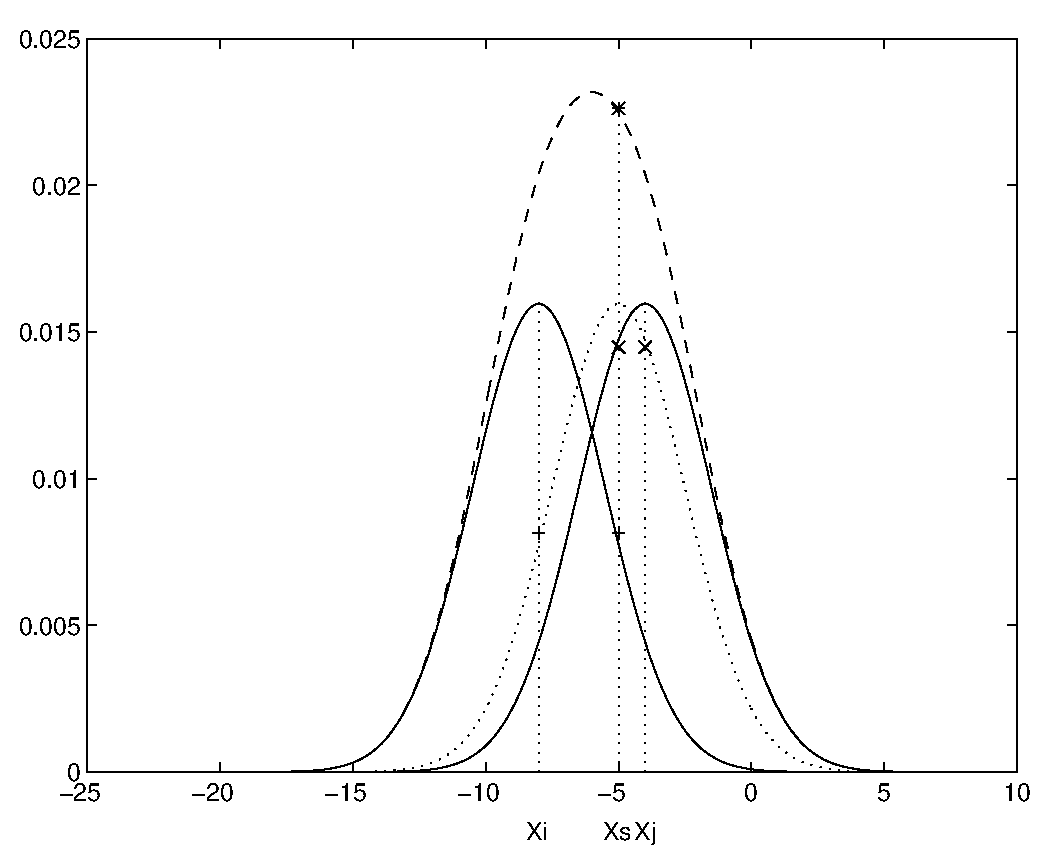
\includegraphics[height=6.5cm]{eijkel2}
  \caption{One kernel at $x_s$ (\emph{dotted kernel}) or two kernels at $x_i$ and $x_j$ (\emph{left and right}) lead to the same summed estimate at $x_s$.
    This shows a figure consisting of different types of lines.
    Elements of the figure described in the caption should be set in italics, in parentheses, as shown in this sample caption. 
    The last sentence of a figure caption should generally end with a full stop, except when the caption is not a full sentence.
  }
  \label{fig:example}
\end{figure}

\begin{figure}[tb]
  \centering
  \begin{subfigure}{0.68\linewidth}
    \fbox{\rule{0pt}{0.5in} \rule{.9\linewidth}{0pt}}
    \caption{An example of a subfigure}
    \label{fig:short-a}
  \end{subfigure}
  \hfill
  \begin{subfigure}{0.28\linewidth}
    \fbox{\rule{0pt}{0.5in} \rule{.9\linewidth}{0pt}}
    \caption{Another example of a subfigure}
    \label{fig:short-b}
  \end{subfigure}
  \caption{Centered, short example caption}
  \label{fig:short}
\end{figure}

If possible (\eg, if you use \LaTeX) please define figures as floating objects. 
\LaTeX{} users, please avoid using the location parameter ``h'' for ``here''. 
If you have to insert a pagebreak before a figure, please ensure that the previous page is completely filled.


\subsection{Formulas}
Displayed equations or formulas are centered and set on a separate line (with an extra line or half line space above and below). 
Equations should be numbered for reference. 
The numbers should be consecutive within the contribution, with numbers enclosed in parentheses and set on the right margin.
For example,
\begin{align}
  \psi (u) & = \int_{0}^{T} \left[\frac{1}{2}
  \left(\Lambda_{0}^{-1} u,u\right) + N^{\ast} (-u)\right] \text{d}t \; \\
& = 0
\end{align}
and 
\begin{equation}
  E = m\cdot c^2.
  \label{eq:important}
\end{equation}
Please do not include section counters in the numbering.

Numbering equations makes reviewing more efficient, because reviewers can refer to a line on a page.  
It is important for readers to be able to refer to any particular equation.
Just because you did not refer to it in the text does not mean some future reader might not need to refer to it.
It is cumbersome to have to use circumlocutions like ``the equation second from the top of page 3''.
(Note that the ruler will not be present in the final copy, so is not an alternative to equation numbers).
All authors will benefit from reading Mermin's description of how to write mathematics:
\url{https://doi.org/10.1063/1.2811173}.

% No color equations in Springer publications.
Equations should never be in color and should be punctuated in the same way as ordinary text.
They should not be pasted in as figures.


\subsubsection{Lemmas, Propositions, and Theorems.}
The numbers accorded to lemmas, propositions, and theorems, \etc should appear in consecutive order, starting with Lemma 1. 
Please do not include section counters in the numbering like ``Theorem 1.1''.


\subsection{Footnotes.}
The superscript numeral used to refer to a footnote appears in the text either directly after the word to be discussed or -- in relation to a phrase or a sentence -- following the punctuation mark (comma, semicolon, or period).%
\footnote{The footnote numeral is set flush left and the text follows with the usual word spacing. 
  Second and subsequent lines are indented. 
}
For remarks pertaining to the title or the authors' names, in the header of a paper, symbols should be used instead of a number.
Please note that no footnotes may be included in the abstract.


\subsection{Cross References}
For the benefit of author(s) and readers, please use the
\begin{verbatim}
  \cref{...}
\end{verbatim}
command for cross-referencing to figures, tables, equations, or sections.
This will automatically insert the appropriate label alongside the cross reference as in this example:
\begin{quotation}
  To see how our method outperforms previous work, please see \cref{fig:example} and \cref{tab:headings}.
  It is also possible to refer to multiple targets as once, \eg~to \cref{fig:example,fig:short-a}.
  You may also return to \cref{sec:intro} or look at \cref{eq:important}.
\end{quotation}
If you do not wish to abbreviate the label, for example at the beginning of the sentence, you can use the
\begin{verbatim}
  \Cref{...}
\end{verbatim}
command. Here is an example:
\begin{quotation}
  \Cref{fig:example} is also quite important.
\end{quotation}


\subsection{Program Code}
Program listings or program commands in the text are normally set in typewriter font (\eg, \texttt{printf("Hello world!\textbackslash{}n");}).


\subsection{Citations}
Arabic numbers are used for citation, which is sequential either by order of citation or by alphabetical order of the references, depending on which sequence is used in the list of references. 
The reference numbers are given in brackets and are not superscript.
Please observe the following guidelines:
\begin{itemize}
\item Single citation: \cite{Authors14}
\item Multiple citation: \cite{Alpher02,Alpher03,Alpher05,Authors14b,Authors14}. 
  The numbers should be listed in numerical order.
  If you use the template as advised, this will be taken care of automatically.
\item If an author's name is used in the text: Alpher \cite{Alpher02} was the first \ldots
\end{itemize}
Please write all references using the Latin alphabet. If the title of the book you are referring to is, \eg, in Russian or Chinese, then please write (in Russian) or (in Chinese) at the end of the transcript or translation of the title.
All references cited in the text should be in the list of references and vice versa.

References should be formatted with the official LNCS reference style.
The \LaTeX{} template already takes care of that through the use of the \texttt{splncs04.bst} Bib\TeX{} style file.
Springer strongly encourages you to include DOIs (Digital Object Identifiers) in your references (\cf \cite{ECCV2022}). 
The DOI is a unique code allotted by the publisher to each online paper or journal article. 
It provides a stable way of finding published papers and their metadata. 
The insertion of DOIs increases the overall length of the references section, but this should not concern you as the reference section is not counted toward the page limit.


\subsection{Miscellaneous}
Compare the following:
\begin{center}
  \begin{tabular}{ll}
    \verb'$conf_a$'          & $\qquad conf_a$ \\
    \verb'$\mathit{conf}_a$' & $\qquad \mathit{conf}_a$
  \end{tabular}
\end{center}
See The \TeX book, p.\ 165.

The space after \eg, meaning ``for example'', should not be a sentence-ending space.
So \eg is correct, \emph{e.g.} is not.
The provided \verb'\eg' macro takes care of this.

When citing a multi-author paper, you may save space by using ``et alia'', 
shortened to ``\etal'' (not ``{\em et.\ al.}'' as ``{\em et\hskip 0.1em}'' is a complete word).
If you use the \verb'\etal' macro provided, then you need not worry about double periods when used at the end of a sentence as in Alpher \etal.
However, use it only when there are three or more authors.
Thus, the following is correct:
   ``Frobnication has been trendy lately.
   It was introduced by Alpher~\cite{Alpher02}, and subsequently developed by
   Alpher and Fotheringham-Smythe~\cite{Alpher03}, and Alpher \etal~\cite{Alpher04}.''

This is incorrect: ``... subsequently developed by Alpher \etal~\cite{Alpher03} ...'' because reference~\cite{Alpher03} has just two authors.


\section{Camera-Ready Manuscript Preparation}
\label{sec:manuscript}
This information will follow after paper decisions have been announced.


\section{Conclusion}
The paper ends with a conclusion. 

\clearpage\mbox{}Page \thepage\ of the manuscript.
\clearpage\mbox{}Page \thepage\ of the manuscript.
\clearpage\mbox{}Page \thepage\ of the manuscript.
\clearpage\mbox{}Page \thepage\ of the manuscript. This is the last page.
\par\vfill\par
Now we have reached the maximum length of an ECCV \ECCVyear{} submission (excluding references).
References should start immediately after the main text, but can continue past p.\ 14 if needed.
\clearpage  % TODO REVIEW/FINAL: This \clearpage needs to be removed from both review and camera-ready versions.


% ---- Bibliography ----
%
% BibTeX users should specify bibliography style 'splncs04'.
% References will then be sorted and formatted in the correct style.
%
\bibliographystyle{splncs04}
\bibliography{egbib}
\end{document}
